%:Clase del documento
\documentclass[fontsize=10pt, Myfinal=true, twoside, numbers=noenddot]{scrbook}
%Minion=true, English=true, Myfinal=true

%:Paquete de estilos propuesto
\usepackage{cabeceras/libroETSI}

%:Paquete específico para cargar tikz (y sus librerías) y pgfplots
\usepackage{cabeceras/dtsc-creafig}

%:Paquete para notaciones específicas
\usepackage{cabeceras/notacion}

%:Paquete para incorporar aspectos concretos de la edición
\usepackage{cabeceras/edicionPFC}


%:Estas líneas de código son INNECESARIAS excepto para mostrar determinadas características en este manual. Pueden eliminarse o comentarse sin ningún problema.
%Se usan para compilar el capítulo estilolibroetsi.tex
\usepackage[final]{showexpl}
\lstset{explpreset={frame=none,rframe={}, numbers=none,numbersep=3pt, columns=flexible,language={[LaTeX]TeX},basicstyle=\ttfamily,keywordstyle=\color{blue}}}%numberstyle=\tiny,

%:Para modificar fácilmente la fuente del texto.
\makeatletter
\ifdtsc@Minion % Queremos utilizar la fuente Minion y lo hemos declarado al principio
	\ifluatex
		\setmainfont[Renderer=Basic, Ligatures=TeX,	% Fuente del texto 
		Scale=1.01,
		]{Minion Pro}
   		% En este caso conviene modificar ligeramente el tamaño de las fuentes matemáticas
		\DeclareMathSizes{10}{10.5}{7.35}{5.25}
		\DeclareMathSizes{10.95}{11.55}{8.08}{5.77}
		\DeclareMathSizes{12}{12.6}{8.82}{6.3}
%		\setmainfont[Renderer=Basic, Ligatures=TeX,	% Fuente del texto 
%		]{Adobe Garamond Pro}
%		\setmainfont[Renderer=Basic, Ligatures=TeX,	% Fuente del texto 
%		]{Palatino LT Std}
	\fi
\else
	\ifluatex
		% Para utilizar la fuente Times New Roman, o alguna otra que se tenga instalada
		\setmainfont[Renderer=Basic, Ligatures=TeX,	% Fuente del texto 
		Scale=1.0,
		]{Times New Roman}
	\else
		\usepackage{tgtermes} 	%clone of Times
		%\usepackage[default]{droidserif}
		%\usepackage{anttor} 	
	\fi
\fi
\makeatother

\usepackage[
    backend=biber,
    sorting=none, 
    %style=authoryear-icomp,
    %sortlocale=de_DE,
    %natbib=true,
    %url=false, 
    %doi=true,
    %eprint=false
]{biblatex}
\defbibheading{etsi}[]{%
        \chapter*{Bibliografía}%
        \chaptermark{Bibliografía} 
        \markboth{#1}{#1}}
\addbibresource{bibliografia.bib}

% Ejemplo de Glosario
\newacronym[type=main]{ETSI}{ETSI}{Escuela Técnica Superior de Ingeniería}
\newacronym[type=main]{US}{US}{Universidad de Sevilla}
\newacronym[type=main]{DMC}{DMC}{Canal Discreto sin Memoria}


\makeindex
\makeglossaries %Si no se quiere el glosario, comentar esta línea.

% Formato A4
\geometry
{paperheight=297mm,%
paperwidth=210mm,%
top=25mm,%
headsep=8.5mm,%
includefoot, 
textheight=240mm, 
textwidth=150mm, 
bindingoffset=0mm, 
twoside}

\usepackage[a4,center]{crop}%para poner las cruces de esquina de página, poner la opción cross

%:Esquema de numeración por defecto
\setenumerate[1]{label=\normalfont\bfseries{\arabic*.}, leftmargin=*, labelindent=\parindent}
\setenumerate[2]{label=\normalfont\bfseries{\alph*}), leftmargin=*}
\setenumerate[3]{label=\normalfont\bfseries{\roman*.}, leftmargin=*}
\setlist{itemsep=.1em}
\setlength{\parindent}{1.0 em}

\setcounter{tocdepth}{4}						% El nivel hasta el que se muestra el índice 

\usepackage{morewrites}
\usepackage[outputdir=build]{minted}
\setminted{fontsize=\footnotesize,linenos,breaklines,mathescape}
\usepackage[minted]{tcolorbox}
\tcbuselibrary{breakable,skins}

\newtcolorbox[auto counter,number within=chapter,list inside={qst}]{codigo}[2][]{,enhanced,breakable, left=1cm,colback=black!5!white,colframe=blue!0!black,fonttitle=\bfseries, title=Código ~\thetcbcounter: #2,#1}
\usepackage{adjustbox}
\usepackage{tikz-3dplot}
%\usepackage{subcaption}
\setcounter{secnumdepth}{40}

\usepackage{gensymb}

\usepackage{pdflscape}
\usepackage{multirow}
\usepackage{placeins}

\makeatletter
\providecommand\add@text{}
\newcommand\tagaddtext[1]{%
     \gdef\add@text{#1\gdef\add@text{}}}% 
     \renewcommand\tagform@[1]{%
          \maketag@@@{\llap{\add@text\quad}(\ignorespaces#1\unskip\@@italiccorr)}%
     }
\makeatother

\begin{document}
%:Para incluir toda la referencia bibliográfica aunque no se cite, descomente la siguiente línea
%\nocite{*}


%PORTADA
%ver edicionPFC.sty para modificaciones
%\mbox{pendiente}
%:Para crear la portada y la portada interior (pagina titular)
\titulo{Posicionamiento de un UAV usando \mbox{marcadores} visuales} %\mbox evita que se divida una palabra al cambiar de línea
\autor{Isidro Jesús Arias Sánchez}
\director{Manuel Vargas Villanueva}
\titulodirector{Profesor Titular}

\departamento{Dpto. de Ingeniería de Sistemas y Automática}
\centro{Escuela Técnica Superior de Ingeniería}
\universidad{Universidad de Sevilla}
\titulacion{Ingeniería Electrónica, Robótica y Automática}
\fecha{2020}
\nombretrabajo{Trabajo de Fin de Master} %Trabajo Fin de Grado, Proyecto fin de Máster,....

\hypersetup
	{
 	linkcolor=black, %Tocar para poner color en enlaces
	pdfauthor={\elautor},
	pdftitle={\nombretrabajo,\eltitulo}, 
	pdfkeywords={Latex, edición, formato de texto}	
	 }

%\portadaPFC{figuras/LogoUS.pdf}{figuras/LogoTSC.pdf} %logo de la Universidad y logo del departamento, si lo hubiera. Para cambiar el pie de página con los logos, debe editarse el fichero ediciónPFC.sty
\portadaPFC{figuras/LogoUS.pdf} %logo de la Universidad y logo del departamento, si lo hubiera. Para cambiar el pie de página con los logos, debe editarse el fichero ediciónPFC.sty

%Fin Portada

\frontmatter
\pagenumbering{Roman} %Pone la numeración en mayúscula (En español parece que es obligatorio)

%\include{dedicatoria/dedicatoria}
% !TEX root =../LibroTipoETSI.tex
\chapter*{Agradecimientos}
%\pagestyle{especial}
\pagestyle{empty}
%\chaptermark{Agradecimientos}
\phantomsection
%\addcontentsline{toc}{listasf}{Agradecimientos}
%\vspace{1cm}
%{\huge{Agradecimientos}}
%\vspace{1cm}

\lettrine[lraise=-0.1, lines=2, loversize=0.25]{E}{stos} 4 años han sido mejores gracias al apoyo de algunas personas. Especialmente quiero agradecérselo a mis padres, Mercedes y José, a mi tía Antonia, a mi abuela Mercedes, a mi hermano Héctor, a Candi, mi novia, a mis amigos de Sevilla, Ángel, Carlos, David, Fernando, Jorge y Samuel, a los de Cádiz, Daniel, Juan Luís, Javier Mena, Javier Sanz, Pepe y Pedro, y por último y no menos importante, a mi tutores Manuel Vargas y Manuel Gil, y al resto de los profesores que me han sabido enseñar y de los que tanto he aprendido. Gracias a todos. 

{\flushleft{\hfill \emph{Isidro Arias Sánchez}}}%
\vspace{-.3cm}
%{\flushleft{\hfill \emph{Estudiante del Grado en Ingenieria Electrónica, Robótica y Mecatrónica}}}%
{\flushleft{\hfill \emph{Sevilla, 2019}}}%


% !TEX root =../LibroTipoETSI.tex
\chapter*{Resumen}
\pagestyle{especial}
\chaptermark{Resumen}
\phantomsection
\addcontentsline{toc}{listasf}{Resumen}

%\lettrine[lraise=-0.1, lines=2, loversize=0.2]{E}{n} este proyecto  se va a desarrollar el  estudio de  un vehículo aéreo no tripulado que tiene dos hélices o rotores orientables, denominado tiltrotor, del ingles \textit{tilt} que significa inclinar.

{\color{red} [Pendiente]}



\chapter*{Abstract}
\pagestyle{especial}
\chaptermark{Abstract}
\phantomsection
\addcontentsline{toc}{listasf}{Abstract}

%\lettrine[lraise=-0.1, lines=2, loversize=0.2]{T}{he} basis of this work is to contribute to the study of a convertible aerial vehicle in which the rotors, being tiltable, operate with the advantages of two different aircraft models, one of the helicopter type that gives it high maneuverability, and one of the airplane type that allows traveling long distances.

{\color{red} [Pendiente]}

 

% Índice abreviado 
% El índice abreviado se incluye también en algunos libros, con menor detalle que el completo. Descomentar las siguientes líneas.
\cleardoublepage
\phantomsection
\addcontentsline{toc}{listasf}{Índice Abreviado}
\pagestyle{especial}
\shorttoc{Índice Abreviado}{1}

%Índice normal, el completo
\cleardoublepage
\phantomsection
\pagestyle{especial}
\tableofcontents


\chapter*{\notationname}
\pagestyle{especial}
\chaptermark{\notationname}
\phantomsection
\addcontentsline{toc}{listasf}{\notationname}
\begin{longtable}{p{3cm}p{8.5cm}}
%TODO: Actualizar la notación de este trabajo
$\bm{P}$ & Posición del vehículo en ejes inerciales  \\
$\bm{V}$ & Velocidad del vehículo en ejes inerciales \\
$\bm{T}$ & Empuje aplicado en ejes cuerpo \\
$\bm{T_{rot}}$ & Empuje aplicado en ejes inerciales \\
$\theta$ &  Inclinación del quadrotor \\
$\bm{\tau}$ &  Par aplicado al quadrotor \\
$\omega$ & Medida del giróscopo \\
$\bm{a}$ & Medida del acelerómetro \\
$R^{UAV\rightarrow C\acute{a}mara}$  & Orientación del marcador vista desde el vehículo\\
$\bm{X}$ &  Vector de estados \\
\end{longtable}
\newpage

\chapter*{Acrónimos}
\pagestyle{especial}
\chaptermark{Acrónimos}
\phantomsection
\addcontentsline{toc}{listasf}{Acrónimos}
\begin{longtable}{p{3cm}p{8.5cm}}
$UAV$ & Vehículo aéreo no tripulado\\
$GCS$ & Estación de control terrestre \\
$NED$ & Ejes norte, este y abajo \\
\end{longtable}
\newpage

 %No incluir si no se quiere, comentándolo

%%:Empieza el contenido del libro
\mainmatter

%:Página por defecto
\pagestyle{esitscCD}
\hypersetup { linkcolor=blue, } 

%% !TEX root =../LibroTipoETSI.tex
%El anterior comando permite compilar este documento llamando al documento raíz
\chapter{Introducción}\label{chp-02}

%\lettrine[lraise=-0.1, lines=2, loversize=0.2]{E}{n} la robótica, uno de los mayores problemas es la percepción del entorno y su ubicación en él. En concreto, cuando se habla de vehículos aéreos no tripulados (UAV), suelen poder posicionarse en el exterior con una precisión de metros. Sin embargo, cuando se trata de navegar en interiores o con precisión más alta el coste de los componentes puede ser muy elevados. Por ejemplo, en exteriores, se puede utilizar la \textit{navegación cinética satelital en tiempo real} (RTK) o en interiores se pueden utilizar balizas acústicas.


%%%%%%%%%%%%%%%%%%%%%%%
\lettrine[lraise=-0.1, lines=2, loversize=0.2]{A}{ctualmente}, los vehículos autónomos no están al alcance de cualquiera. Estos no deben de confundirse con los vehículos no tripulados, como los UAVs (Vehículos aéreos no tripulados) que si están más extendidos, llegando a utilizarse para ocio o para negocios estando al alcance del bosillo de cada vez más gente. La mayoría tienen una autonomía parcial y necesitan la supervisión de un piloto en algunas de sus fases de vuelo, como por ejemplo en el aterrizaje o cuando se navega cerca de obstáculos. Además muchos de ellos solo pueden volar en exteriores donde le llega la señal de los satélites. 
La causa de todas estás limitaciones está en que no pueden determinar dónde están ubicados con exactitud y que la precisión que sulelen tener es de varios metros. Si se mejorase ese aspecto, el número de aplicaciones en las que se podría utilizar sería enorme. 
Por ejemplo, se podría programar un vuelo de reconocimiento cuando se detecte un intruso en una propiedad. También perimitiría manipular objetos como la recogida y depósito de paquetes.  

% Autonomo permite:
% - que no tengan experiencia
% - que se pueda activar las 24 horas del día sin nadie pendiente
% - que sea escalable
% - Si existe una base es más inmediato
El interés de realizar estas tareas de forma autónoma no solo está en que cualquiera pueda hacer uso del vehículo, sin necesitar licencia ni habilidades especiales, si no que también hace el sistema más escalable. Si se quisiera por ejemplo, instalar un sistema de reparto de paquetes mediante vehículos aéreos, y la flota es cada vez más grande, llegará un momento que sea dificil que todos los pilotos se pongan de acuerdo compartiendo el mismo espácio aéreo. Si esta planificación la hace en su lugar un ordenador, posiblemente el sistema sea más optimo. Como última ventaja de la automatización se podría decir que el vehículo podría estar disponible de forma inmediata en cualquier momento y no obligaría a las personas a estar trabajando en horas de descanso. 

%Existen formas pero son más caras:
Si se disponen de los suficientes recursos existe la tecnología para conseguirlo, por ejemplo mediante balizas sonoras, que son usadas en interiores de fábricas o si se opera en el exterior, existe la posibilidad de  \textit{navegación cinética satelital en tiempo real} (RTK). Otra solución que no necesita de instalación en el entorno, son las cámaras o lídares, que con el uso de unos algoritmos llamados SLAM, pueden crear un mapa del entorno y ubicarse en él. El problema de estos es que o bien sus sensores son caros o bien tienen una alta carga computacional que obligan a instalar grandes y costosos ordenadores a bordo del vehículo. 

\begin{figure}[b]
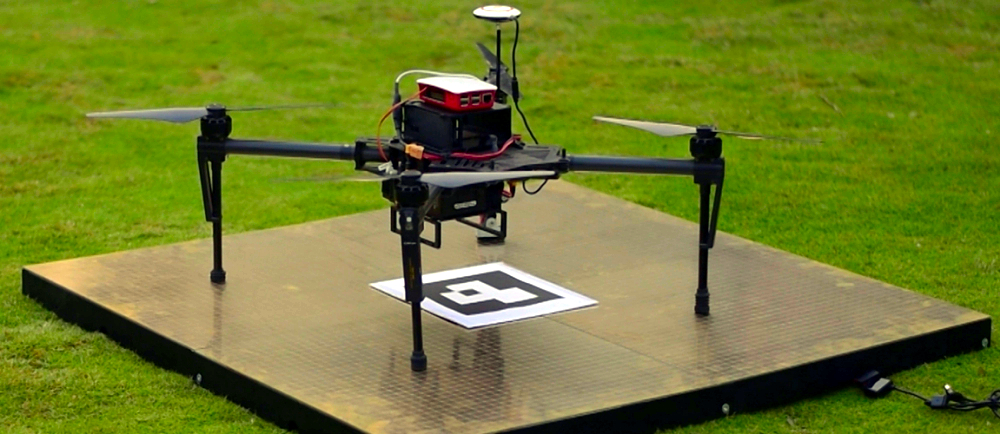
\includegraphics[width=0.7\textwidth]{introduccion/flytbase_en.jpg}
\caption{Estación de carga de \textit{Flytbase}}
\label{fig:flyt}
\end{figure}

%La alternativa: marcadores visuales
Lo que se busca en este trabajo es una alternativa más barata que consiga un posicionamiento centimétrico del vehículo. En concreto se ha hecho uso de unos marcadores visuales planos. Estos contienen figuras que son fácilmente detectables procesando una imagen de dicho marcador, por ejemplo los contornos de un cuadrilátero. Además, para su procesamiento se usará uno de los ordenadores embebidos más baratos del mercado 
% facil de imprimir, requiere menos computo, puede llegar a ser muy robusto. 
% Marcadores visuales. Solución robusta (no hay muchos falsos positivos) ya que es complicado encontrarse en el entorno algo parecido (no como los que usan una pelota), y además barata ya que tiene poco costo computacional, al contrario que los SLAM por ejemplo. 

 
% Implementaciones comerciales
Ya están a la venta algunas soluciones que utilizan esta tecnología para el aterrizaje automático. En concreto algunas  empresas como \textit{Everdrone} \cite{everdrone} y \textit{Flytbase} (ver figura \ref{fig:flyt}) ofrecen estaciones de carga con los mismos marcadores utilizados aquí. 

% Papers
Existen articulos en los que ya han utilizado marcadores visuales para mejorar el posicionamiento de un UAV, la mayoría teniendo como objetivo el aterrizaje automático. En \cite{sani2017automatic} se consigue que un quadrotor \textit{Parrot AR.Drone} aterrice sobre un marcador Aruco, incluso si brevemente se pierde la vista al marcador utilizando las medidas de la IMU. En \cite{yang2015precise} además de la IMU, se utiliza un sensor de flujo óptico para conseguir aterrizar el vehículo. En ninguno de los dos trabajos se utiliza un autopiloto de código abierto, sino se limitan a utilizar las interfaces de programación que aportan Parrot y DJI respectivamente para tomar las medidas de los sensores y comandarle una postura de referencia. 
Además, la falta de detalles de implementación que suele haber en este tipo de artículos, hace que su trabajo sea más dificil de ser repetido por el lector.
En este proyecto, lo que se quiere aportar otro enfoque en el que se hace uso del estimador de estados del autopiloto, el mismo que se utiliza para estimar la orientación y al que le llegan las medidas de la IMU, magnetómetro, barómetro, etc., para obtener una fuente precisa de posición.  
%Esa fusión de las medidas se realiza en el mismo autopiloto, y no en un ordenador externo, con la idea de que los retrasos en las comunicaciones tengan menor efecto. 

% Los puntos que se veran
En este trabajo en primer lugar, en el capítulo \ref{chp:est} se hace un estudio de una parte clave para el posicionamiento con marcadores, que es el estimador de estados. Además se elabora y se muestran los resultados de una simulación en la que se pone a prueba este. En el capítulo \ref{chp:pos} se explica cómo se ha implementado este posicionamiento, mostrando los componentes utilizados y explicando el programa creado. Finalmente, en ese mismo capítulo se enseñan los resultados experimentales a los que se ha llegado.  



\endinput

% !TEX root =../main.tex
\chapter{Estimador de estados}\label{chp:1}

\lettrine[lraise=-0.1, lines=2, loversize=0.2]{E}{n} este capítulo se analizará uno de los elementos que se utilizarán en el siguiente, que es el estimador de estados. En concreto se analiza el que incorpora el autopiloto de código abierto PX4, ya que será este se utilizará para la implementación. Previamente, en \cite{arias2019control} se hizo una explicación parcial de este, pero se dejaron atrás algunos detalles como el manejo de las medidas retrasadas. Aquí se explicará esto y además se realizará una simulación que demuestre la eficacia del algoritmo.

\section{Manejo de medidas retrasadas}
En muchas ocasiones se tienen sensores con un retraso muy diferentes entre ellos, por ejemplo una IMU es mucho más rápida que el procesamiento de la imagen de una cámara o el GNSS. PX4 lo soluciona añadiendo más elementos a la estructura original de un estimador de estados. Uno de sus elementos es un \textit{Filtro de Kalman Extendido} (EKF). Este no usa las medidas más nuevas que le llegan, si no que las almacena y utiliza las que llegaron hace un determinado tiempo. Corriendo en paralelo, existe un estimador llamado \textit{Filtro de Salida}, el cual sí que utiliza la última medida del acelerómetro y del giróscopo. 

% TODO: Plantear los sensors y que da igual su periodos
% TODO: decir que el periodo de muestreo es de 5 ms

Supongamos que se tiene un sistema que se mueve en el espacio y del que se quiere conocer sus estados, en concreto, su posición, su velocidad y su orientación. Para este objetivo el sistema está dotado de numerosos sensores como que son un acelerómetro, un giróscopo, un barómetro, un GNSS o un sensor de flujo óptico. Cada uno de ellos tiene diferentes propiedades en cuanto a retraso, ruido, precisión, etc. Por ejemplo, la medida aportada por el GNSS es la única fuente de posición absoluta, sin embargo, tiene un gran retraso y las medidas que genera se refieren a la posición que se tenía hace un tiempo (generalmente decenas de milisegundos). 

Para explicar un método de cómo afrontar  este problema, se va a poner un ejemplo de la ejecución paso a paso del estimador de estados con diferentes sensores.
Supongamos que en el primera ejecución del estimador, se toma la primera medida de la IMU (acelerómetro y giróscopo). El EKF todavía no la utiliza, si no que la guarda en su buffer (figura \ref{fig:est1}). Conforme llegan nuevas medidas, que ocurre cada 5 ms, estas se introducen en la posición de más a la izquierda del buffer y las que ya estaban se van desplazando hacia la derecha, hasta que llegan a la última celda. La medidas de esta celda situada más a la derecha, son las que son usadas por el EKF. Los estados que este genera y las medidas utilizadas para estimarlos se refieren al \textit{horizonte de tiempo retrasado}. Como se muestra en la figura, el buffer tiene una longitud de 7 celdas, por lo tanto las medidas de la IMU que llegan al EKF siempre serán las que se recogieron hace 30 ms.  

\begin{figure}	
	\centering
	\begin{subfigure}[t]{0.9\textwidth}
		\centering
		\hspace*{-2.0cm}
		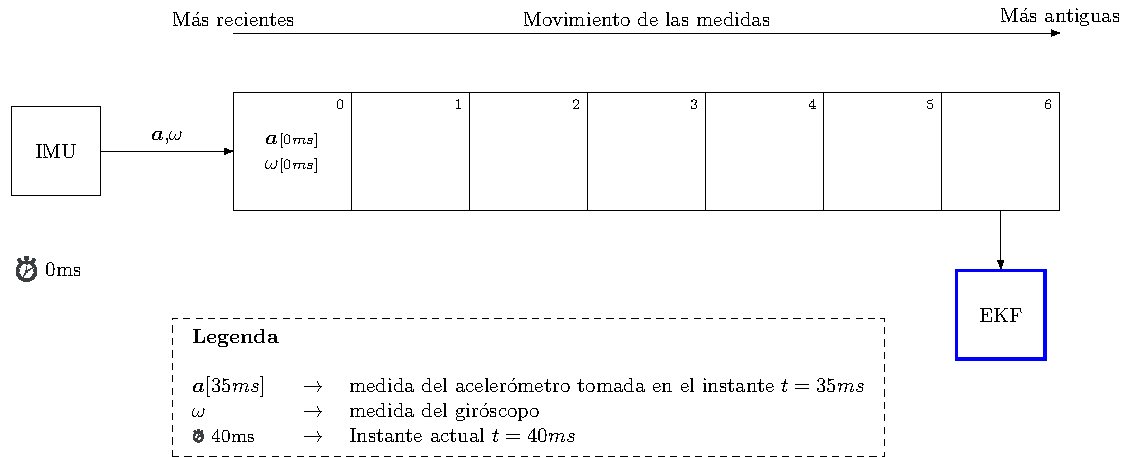
\includegraphics[width=\textwidth]{estimador_px4/tikz/ekf_output_1}
		\caption{Primera medida tomada de la IMU}\label{fig:est1}		
	\end{subfigure}
	\quad
	\begin{subfigure}[t]{1.05\textwidth}
		\centering
		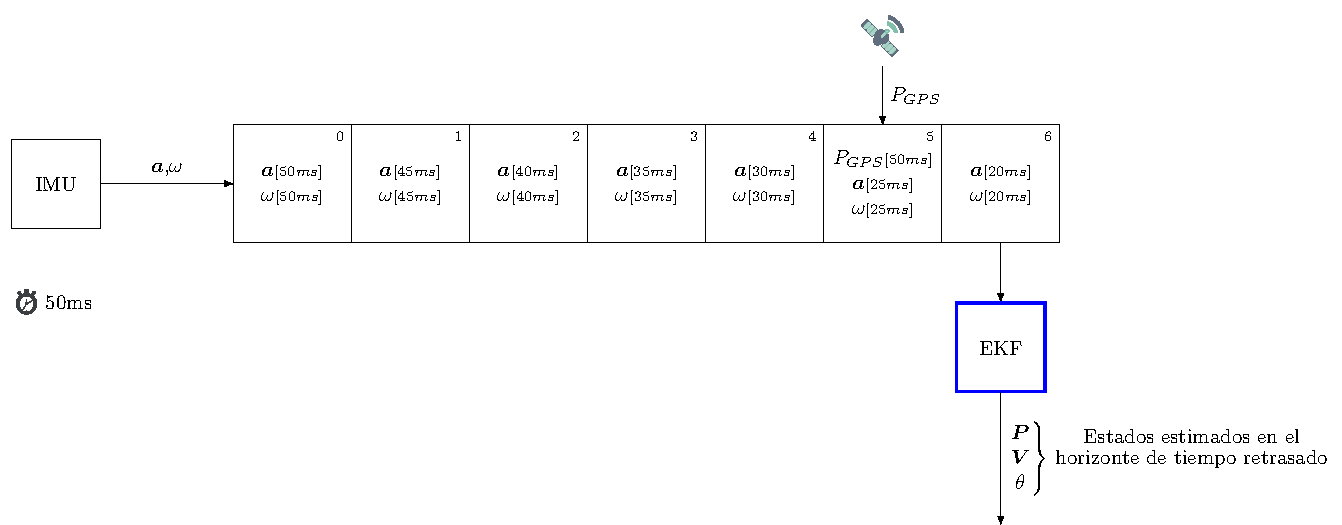
\includegraphics[width=\textwidth]{estimador_px4/tikz/ekf_output_2}
		\caption{Llegada de la medida del GPS}\label{fig:est2}		
	\end{subfigure}
	\begin{subfigure}[t]{0.9\textwidth}
		\centering
		\vspace{1cm}
		\hspace*{-2cm}
		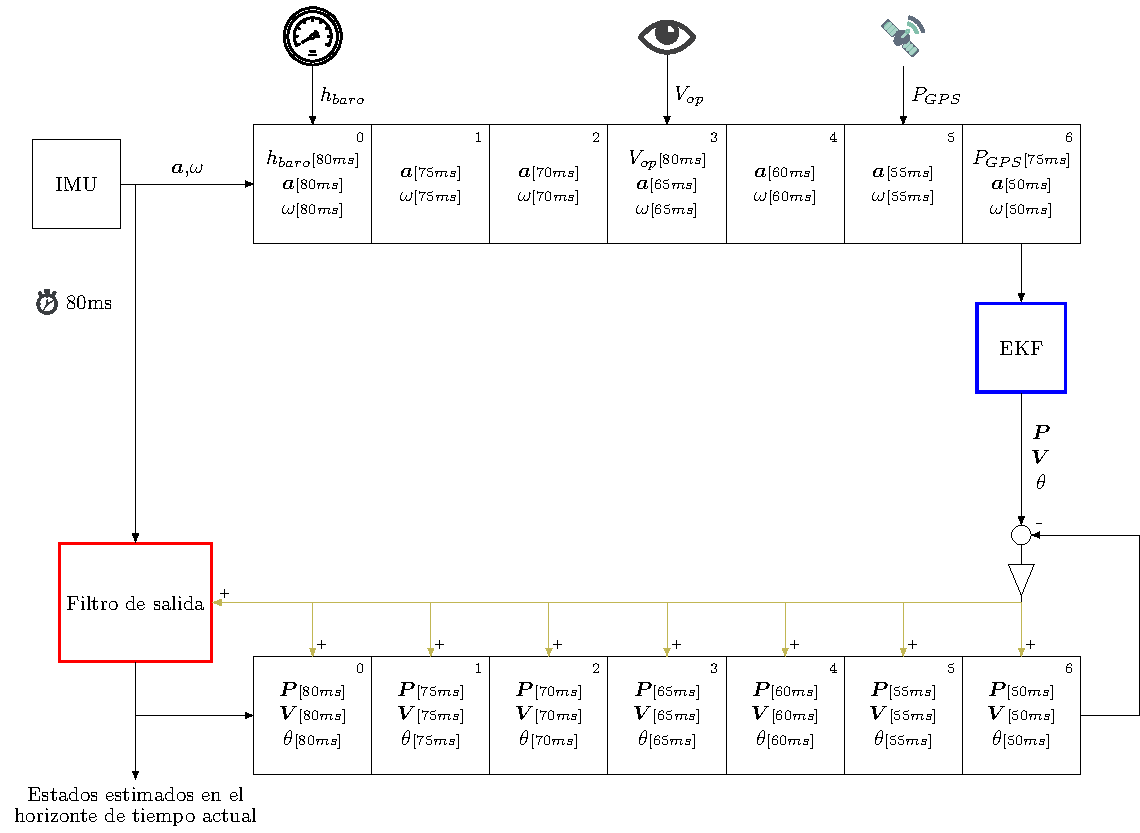
\includegraphics[width=\textwidth]{estimador_px4/tikz/ekf_output_3}
		\caption{Estimador completo}\label{fig:est3}		
	\end{subfigure}
	\quad
	\caption{Manejo de medidas retrasadas}\label{fig:retraso}
\end{figure}

Pasan algunos ciclos más hasta que en el instante 60ms llega la primera medida del GPS, pero esta no se coloca en el extremo izquierdo del buffer junto con las medidas más recientes de la IMU, si no que se lleva directamente a la celda número 5 (ver figura \ref{fig:est2}). En esta también se encuentran las medidas de la IMU tomadas en el instante 35ms, es decir las que fueron tomadas hace 25 ms, que coincide con el retraso que tiene la posición del GPS con respecto a la IMU o lo que es lo mismo, la medida del GPS, corresponde a la posición que tenía el vehículo hace 25 ms. De esta manera se agrupan las medidas que se refieren al mismo instante físico, es decir, el instante en el que llegaron pero {\bfseries compensándose su retraso}. 


De forma paralela se ejecuta el \textit{filtro de salida}, que es otro estimador de estados y para esta explicación se va a suponer que su funcionamiento interno es exactamente igual al del EKF, la única diferencia es que solamente utiliza las medidas de la IMU, en este caso las que se generan más recientemente. Estos estados se refieren al \textit{horizonte de tiempo actual} y son los únicos que se usan para las otras tareas que tenga vehículo, como por ejemplo para alimentar al controlador de orientación, por esta razón se le denomina filtro de salida. El problema que tiene este es que desaprovecha todos los demás sensores que tiene el vehículo, por lo que se le aplica un \textbf{mecanismo de corrección}.  

Este mecanismo está compuesto otro buffer llamado \textit{buffer de salida}, que se comporta de la misma manera que el primero, pero en lugar de guardar medidas, almacena los estados del filtro de salida. Estos estados se van desplazando hacia la derecha hasta que llegan a la última posición del buffer. En esta posición están los estados que se estimaron por el filtro de salida hace 30 ms, que coincide con el retraso que tienen las medidas del la IMU que entran al EKF. Si al EKF solo se le hubiese suministrado las medidas de la IMU, al igual que al filtro de salida, los estados del EKF y los que hay almacenado en esta última celda del buffer de salida coincidirían. Sin embargo, lo que está ocurriendo es que el EKF recoge medidas de otros sensores y por lo tanto no coincidirán. Para realizar la corrección, se calcula la diferencia entre ellos. Esta diferencia se atenúa y se le suma a todos los elementos del buffer de salida, además de al propio filtro de salida. 

En la figura \ref{fig:est3} se ha ilustrado este mecanismo de correción además de incluir más medidas: la velocidad proporcionada por flujo óptico ($V_{op}$), la cual tiene un retraso de 15ms, y la altura que proporciona el barómetro, que se ha supuesto que no tiene ningún retraso. 

% TODO: comentar otras medidas que han llegado




\subsection{Detalles de implementación}
% tamaño de los buffer
En este apartado se presentan algunos trozos de código de PX4 que implementan lo anteriormente descrito más algunos detalles que he se han omitido en el apartado anterior para que fuese más fácil su comprensión.

En el apartado anterior se explicó que la error entre los estados estimados en el horizonte de tiempo retrasado y los estados del buffer de salida, se atenuaban (multiplicar por una ganancia menor que 1, mostrado en la figura \ref{fig:est3} como un triángulo) y se le suma a todo el buffer de salida. En el siguiente código se puede ver cómo se ha implentado esto. Se puede ver que la correción de la velocidad y la posición no solo se calcula a partir del error, sino también a partir de la integral del error, por lo tanto aqui se tiene un control proporcional-integral que tiene como señal de control la correción al buffer de salida. De esta manera, los estados en el horizonte de tiempo actual, se igualarán a los del horizonte de tiempo retrasado en régimen permanente. 

\begin{codigo}{Correción del buffer de salida. Ubicado en  la línea \href{https://github.com/PX4/PX4-ECL/blob/ec934908900b23ee273d1a9f82364b7b38423200/EKF/ekf.cpp\#L488}{488} del archivo \textit{Firmware/src/lib/ecl/EKF/ekf.cpp}}
\begin{minted}[firstnumber=488]{c++}
void Ekf::applyCorrectionToOutputBuffer(float vel_gain, float pos_gain){
	// calculate velocity and position tracking errors
	const Vector3f vel_err(_state.vel - _output_sample_delayed.vel);
	const Vector3f pos_err(_state.pos - _output_sample_delayed.pos);

	_output_tracking_error(1) = vel_err.norm();
	_output_tracking_error(2) = pos_err.norm();

	// calculate a velocity correction that will be applied to the output state history
	_vel_err_integ += vel_err;
	const Vector3f vel_correction = vel_err * vel_gain + _vel_err_integ * sq(vel_gain) * 0.1f;

	// calculate a position correction that will be applied to the output state history
	_pos_err_integ += pos_err;
	const Vector3f pos_correction = pos_err * pos_gain + _pos_err_integ * sq(pos_gain) * 0.1f;

	// loop through the output filter state history and apply the corrections to the velocity and position states
	for (uint8_t index = 0; index < _output_buffer.get_length(); index++) {
		// a constant velocity correction is applied
		_output_buffer[index].vel += vel_correction;

		// a constant position correction is applied
		_output_buffer[index].pos += pos_correction;
	}

	// update output state to corrected values
	_output_new = _output_buffer.get_newest();
}
\end{minted}
\end{codigo} 

En el código anterior no ha aparecido la correción de la orientación, y esto es porque requieren que sea tratada a parte. En este estimador, la orientación se expresa en cuaternios y la operación de la correción no es simplemente una suma como ocurría en el caso de la velocidad, es más complicada y se tardaría demasiado en aplicarla a todos los elementos del buffer. En su lugar, únicamente se aplica una correción a la orientación estimada en el horizonte de tiempo actual.

\begin{codigo}{Correción de la orientación. Ubicado en el archivo \textit{Firmware/src/lib/ecl/EKF/ekf.cpp}}
En la línea \href{https://github.com/PX4/PX4-ECL/blob/ec934908900b23ee273d1a9f82364b7b38423200/EKF/ekf.cpp\#L323}{323} se corrige la orientación:
\begin{minted}[firstnumber=323]{c++}
  // Apply corrections to the delta angle required to track the quaternion states at the EKF fusion time horizon
  const Vector3f delta_angle(imu.delta_ang - _state.delta_ang_bias * dt_scale_correction + _delta_angle_corr);
\end{minted}
En la línea \href{https://github.com/PX4/PX4-ECL/blob/ec934908900b23ee273d1a9f82364b7b38423200/EKF/ekf.cpp\#L411}{411} se calcula la ganancia del control
\begin{minted}[firstnumber=411]{c++}
    // calculate a gain that provides tight tracking of the estimator attitude states and
    // adjust for changes in time delay to maintain consistent damping ratio of ~0.7
    const float time_delay = fmaxf((imu.time_us - _imu_sample_delayed.time_us) * 1e-6f, _dt_imu_avg);
    const float att_gain = 0.5f * _dt_imu_avg / time_delay;
    
    // calculate a corrrection to the delta angle
    // that will cause the INS to track the EKF quaternions
    _delta_angle_corr = delta_ang_error * att_gain;
\end{minted}
\end{codigo} 

%La ganancia que multiplica la diferencia entre el filtro de salida y el EKF y que sirve para corregir los estados, se calcula de manera el sistema controlado tenga un factor de amortiguamiento de 0.7.
%\begin{equation}
%K_p=\frac{0.5}{Retraso}
%\end{equation} 
%Puede que este valor se haya sacado de aproximar un retraso e^{sT} por un padé, como viene en https://www.researchgate.net/publication/237396133_RATIONAL_APPROXIMATION_OF_TIME_DELAY
% sin embargo no se como sacar el factor de amortiguamiento de funciones de tranferencia con ceros de fase no mínima.

% TODO: Tamaño del buffer. 
% TODO: buffer de salida se ejecuta más frecuentemente. 
En el siguiente código se puede ver cómo se calcula la logitud del buffer de las medidas de la IMU. Se puede ver que se hace para que haya espacio para medidas que tengan un retraso igual al sensor que más retraso tiene.
\begin{codigo}{Cálculo del tamaño del buffer. Ubicado en el archivo \textit{Firmware/src/lib/ecl/EKF/estimator\_interface.cpp}}
\begin{minted}[firstnumber=512]{c++}
  // find the maximum time delay the buffers are required to handle
  const uint16_t max_time_delay_ms = math::max(_params.mag_delay_ms,
  				     math::max(_params.range_delay_ms,
  				       math::max(_params.gps_delay_ms,
  					 math::max(_params.flow_delay_ms,
  					   math::max(_params.ev_delay_ms,
  					     math::max(_params.auxvel_delay_ms,
  					       math::max(_params.min_delay_ms,
  						 math::max(_params.airspeed_delay_ms,
  						       _params.baro_delay_ms))))))));
  
  // calculate the IMU buffer length required to accomodate the maximum delay with some allowance for jitter
  _imu_buffer_length = (max_time_delay_ms / FILTER_UPDATE_PERIOD_MS) + 1;
\end{minted}
\end{codigo} 


\section{EKF para modelo bidimensional}
Se buscará un modelo discreto de espacio de estados descrito de la siguiente manera:
\begin{align}
X_{k+1} =  f(X_k)
\end{align}

Se va aplicar a un quadrotor en 2 dimensiones, pero el modelo al ser cinemático, se podría aplicar a cualquier otro móvil.

Estados:
\begin{align}
X = 
\begin{bmatrix} 
x \\ y \\ V_x \\ V_y \\ \theta
\end{bmatrix}
\end{align}

Modelo de predicción cinemático:
\begin{align}
\begin{bmatrix} 
x \\ y 
\end{bmatrix}_{k+1}
=
\begin{bmatrix} 
x \\ y 
\end{bmatrix}_k
+
\begin{bmatrix} 
V_x \\ V_y 
\end{bmatrix}_k
\Delta t
\end{align}

\begin{align}
\begin{bmatrix} 
V_x \\ V_y 
\end{bmatrix}_{k+1}
=
\begin{bmatrix} 
V_x \\ V_y 
\end{bmatrix}_k + 
\Delta t
\begin{bmatrix} 
\cos{\theta} & \sin{\theta} \\ -\sin{\theta} & \cos{\theta}
\end{bmatrix}
\bm{a} +  
\begin{bmatrix} 
0 \\ - m\ g 
\end{bmatrix}\Delta t
\end{align}

\begin{align}
\theta_{k+1} = \theta_k + \Delta t \omega
\end{align}


Jacobiano del modelo de predicción:
\begin{align}
F =\left. \frac{\partial f}{\partial X}\right| _{X_{k-1}} =  
\begin{bmatrix} 
%x/X
1 	&0	&\Delta t	&0		&0\\
%y/X
0 	&1	&0		&\Delta t	&0\\
%Vx/X
0 	&0	&1		&0		&\Delta t\left(-a_x\sin{\theta_{k-1}} + a_y\cos{\theta_{k-1}}\right) \\
%Vy/X
0 	&0	&0		&1		&\Delta t\left(-a_x\cos{\theta_{k-1}} - a_y\sin{\theta_{k-1}}\right) \\
%theta/X
0 	&0	&0		&0		&1
\end{bmatrix}
\end{align}

Jacobiano del modelo de predicción con respecto a la aceleración a la velocidad angular. 
\begin{align}
G =  \frac{\partial f}{\partial \bm{a},\omega} = 
\begin{bmatrix} 
%x/a,w
0 			&0			&0\\
%y/a,w
0 			&0			&0\\
%Vx/a,w
\Delta t \cos{\theta} 	&\Delta t \sin{\theta}	&0\\
%Vy/a,w
-\Delta t \sin{\theta} 	&\Delta t \cos{\theta}	&0\\
%theta/a,w
0 			&0			&\Delta t		
\end{bmatrix}
\end{align}

Matriz de covarianzas de la predicción:
\begin{align}
Q = 
G
\begin{bmatrix} 
\sigma^2_a 	& 0 		& 0\\
0 		& \sigma^2_a 	& 0\\
0 		& 0 		& \sigma^2_\omega\\
\end{bmatrix}
G^T
\end{align}
Donde $\sigma^2_a$ y $\sigma^2_\omega$ son las varianzas del acelerómetro y del giróscopo, que se pueden hayar experimentalmente o viendo la hoja de datos de los sensores. 

\section{Simulación del quadrotor y del estimador}
En este apartado se implementará el filtro explicado en este capítulo y pondrá a prueba con un simulador de un quadrotor. Tanto el estimador como el simulador estarán programados en lenguaje python. El simulador será muy sencillo, describirá el movimiento de un quadrotor en el plano al que únicamente se le aplican la fuerza de la gravedad, un empuje y un par. Estos dos últimos se serán generados por un controlador de velocidad vertical y un controlador de ángulo, los cuales toman la velocidad, y la inclinación real del vehículo en lugar de medidas ruidosas. Sus referencias se han escogido para que desde el reposo, ascienda unos metros, y luego se desplace hacia la dirección negativa del eje x. 


\begin{figure}
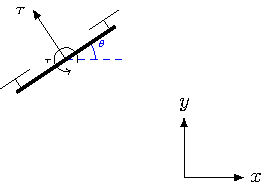
\includegraphics[width=0.5\textwidth]{estimador_px4/tikz/quadrotor_2d}
\caption{Quadrotor en dos dimensiones}
\label{fig:model}
\end{figure}

Para simular el quadrotor se realiza una integración discreta de la segunda ley de Newton:
\begin{align}
        \ddot{\theta} &= \frac{\tau}{I} \\
        \dot{\theta} &= \dot{\theta}_{i-1} + \Delta t \ddot{\theta} \\
        \theta &= \theta_{i-1} + \Delta t \dot{\theta} \\
        R &= 
\begin{bmatrix}
\cos{\theta}& -\sin{\theta}\\
\sin{\theta} & \cos{\theta}
\end{bmatrix}\\
         \bm{T_{rot}}&= R  \begin{bmatrix}0\\ T \end{bmatrix}\\
         \bm{F_g}&= \begin{bmatrix}0\\ -m g \end{bmatrix}\\
         \bm{a}& = \frac{\bm{T_{rot}}+\bm{F_g}}{m}\\
         \bm{v}& = v_{i-1} + \bm{a}\Delta t  \\
        \bm{p} &= p_{i-1} + \bm{v}\Delta t  \\
\end{align}


Una vez se ha simulado esta trayectoria, se pasa ejecutar el estimador de estados. Este toma unas medidas a las que se le ha aplicado un ruido gaussiano y genera su estimación de los estados. Finalmente estos se comparan con los estados reales y se verifica el desempeño del estimador. 

El primer experimento que se va a mostrar, al estimador de estados no le va a entrar ninguna otra medida que no sea la del giróscopo y la del acelerómetro. En la figura \ref{fig:simu1} se puede apreciar que la estimación de la posición tiene una deriva, ya que no hay ningún sensor que aporte posición absoluta. 

\begin{figure}[b]
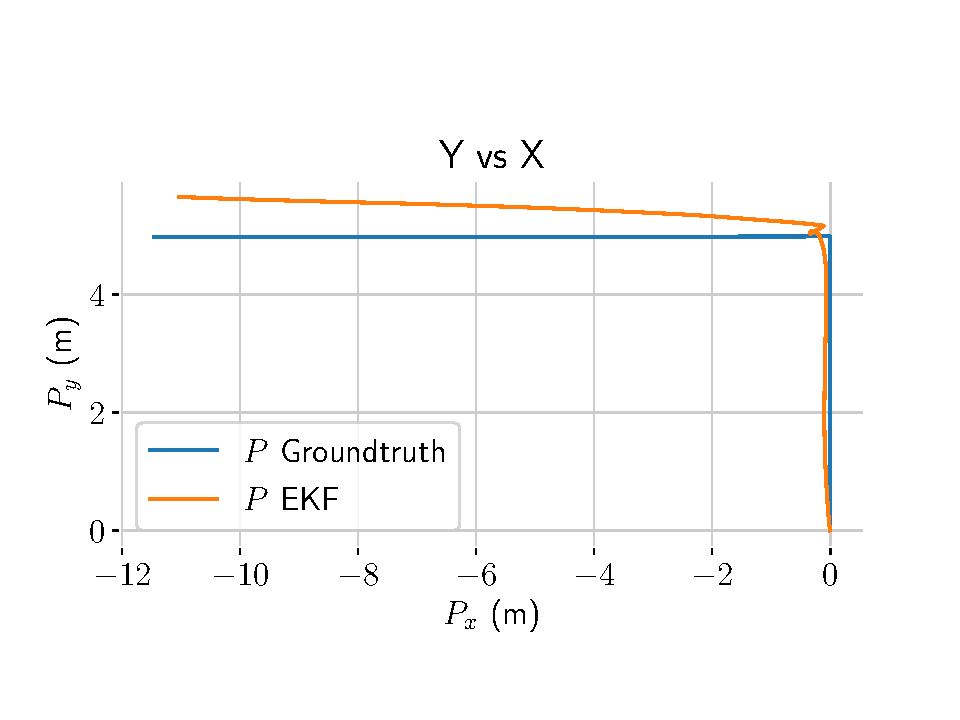
\includegraphics[width=0.5\textwidth]{estimador_px4/im_simu/n_update/tray}
\caption{EKF no ejecuta la fase de actualización}
\label{fig:simu1}
\end{figure}


En el siguiente experimento se va a fusionar un GPS con un retraso de 1 segundo. Este valor es poco relista pero de esta manera se aprecia más la degradación de la estimación. Se puede ver en la figura \ref{fig:no-handle} que el GPS emperora la estimación, ya que en el instante $t=1s$, la estimación se aleja de su valor real porque llega la primera medida del GPS. 
\begin{figure}	
	\centering
	\hspace*{-0.5cm}
	\begin{subfigure}[t]{0.49\textwidth}
		\centering
		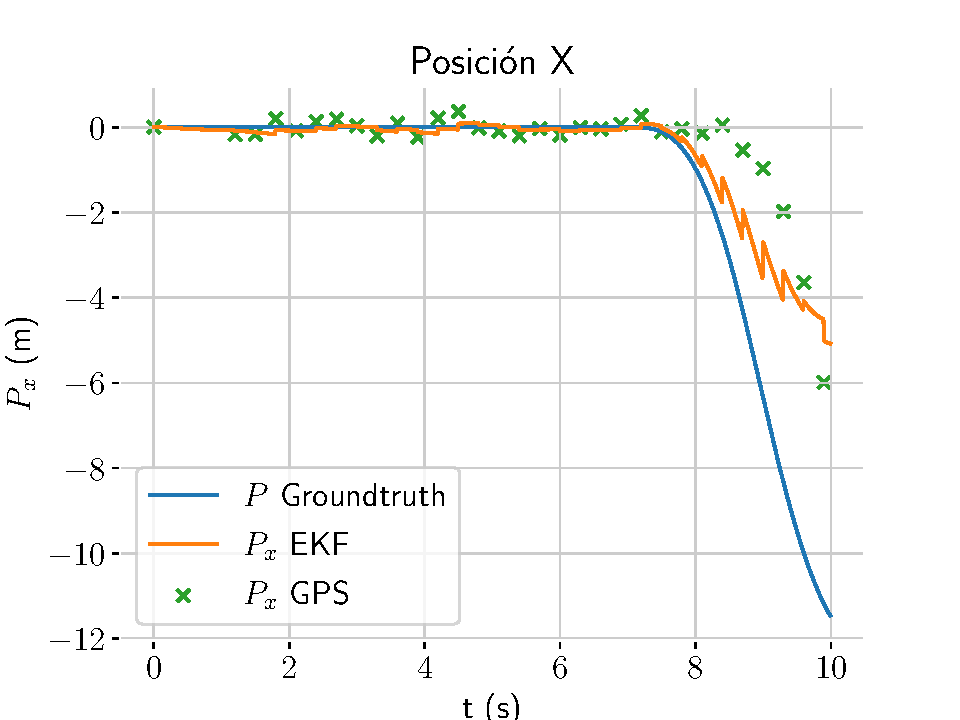
\includegraphics[width=\textwidth]{estimador_px4/im_simu/no_handle_delay/x_t}
		\caption{}
		\label{fig:no-handle-xt}		
	\end{subfigure}
	\quad
	\begin{subfigure}[t]{0.49\textwidth}
		\centering
		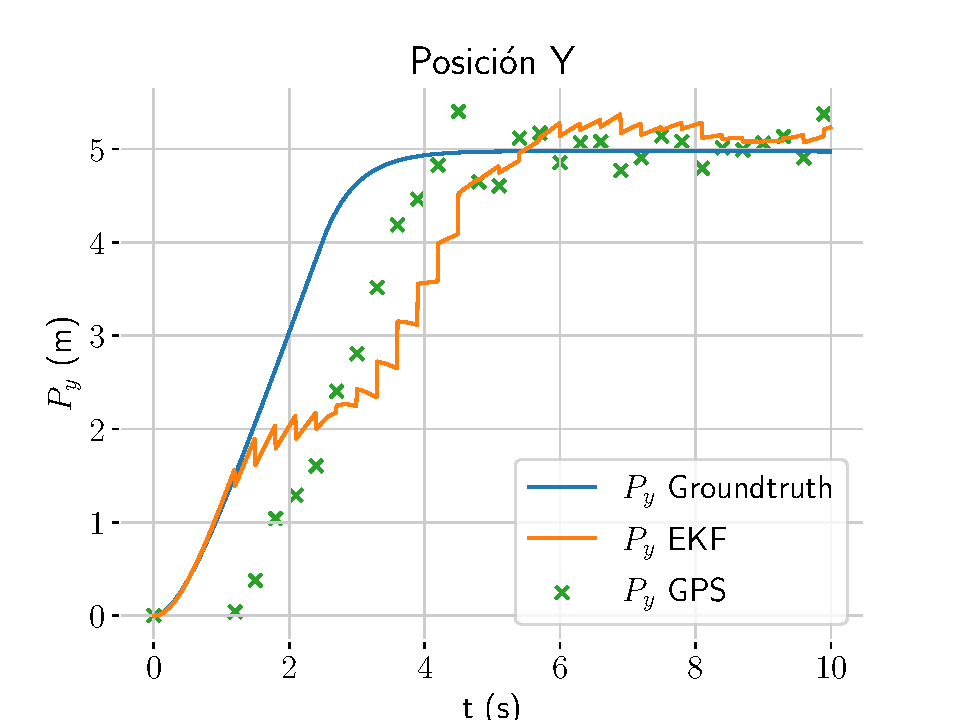
\includegraphics[width=\textwidth]{estimador_px4/im_simu/no_handle_delay/y_t}
		\caption{}
		\label{fig:no-handle-yt}		
	\end{subfigure}
	\quad
	\hspace*{-0.5cm}
	\begin{subfigure}[t]{0.49\textwidth}
		\centering
		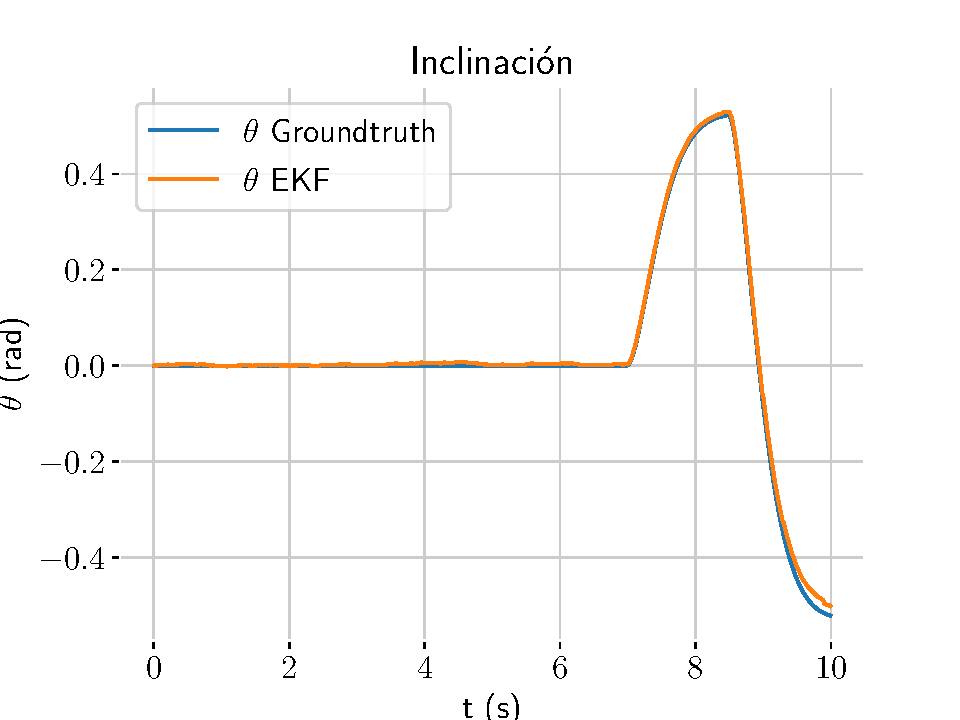
\includegraphics[width=\textwidth]{estimador_px4/im_simu/no_handle_delay/theta}
		\caption{}
		\label{fig:no-handle-theta}		
	\end{subfigure}
	\quad
	\begin{subfigure}[t]{0.49\textwidth}
		\centering
		\includegraphics[width=\textwidth]{estimador_px4/im_simu/no_handle_delay/vx}
		\caption{}
		\label{fig:no-handle-vx}		
	\end{subfigure}
	\quad
	\caption{Fusión del GPS con retraso}\label{fig:no-handle}
\end{figure}

En el tercer experimento se realizar el manejo de los retrasos explicado en este capítulo. En la figura \ref{fig:handle} se tiene que, aunque la estimación esté retrasada un segundo, esta no se ve degradada por el GPS ya que se le está compensando su retraso antes de fusionarlo con las medidas de la IMU. 

\begin{figure}	
	\centering
	\hspace*{-0.5cm}
	\begin{subfigure}[t]{0.49\textwidth}
		\centering
		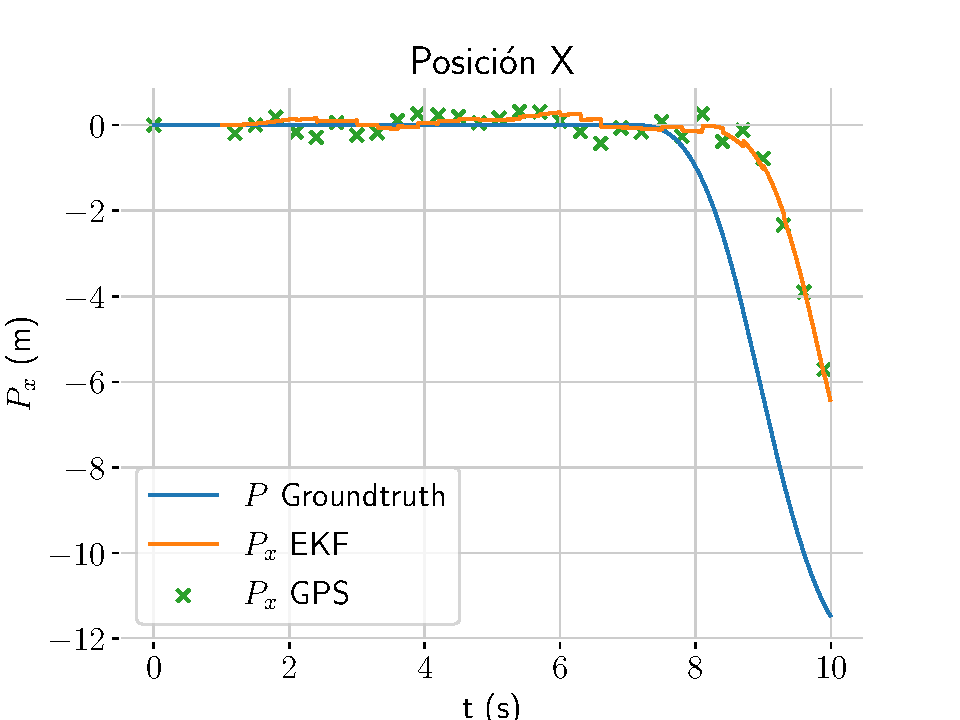
\includegraphics[width=\textwidth]{estimador_px4/im_simu/handle_delay/x_t}
		\caption{}
		\label{fig:handle-xt}		
	\end{subfigure}
	\quad
	\begin{subfigure}[t]{0.49\textwidth}
		\centering
		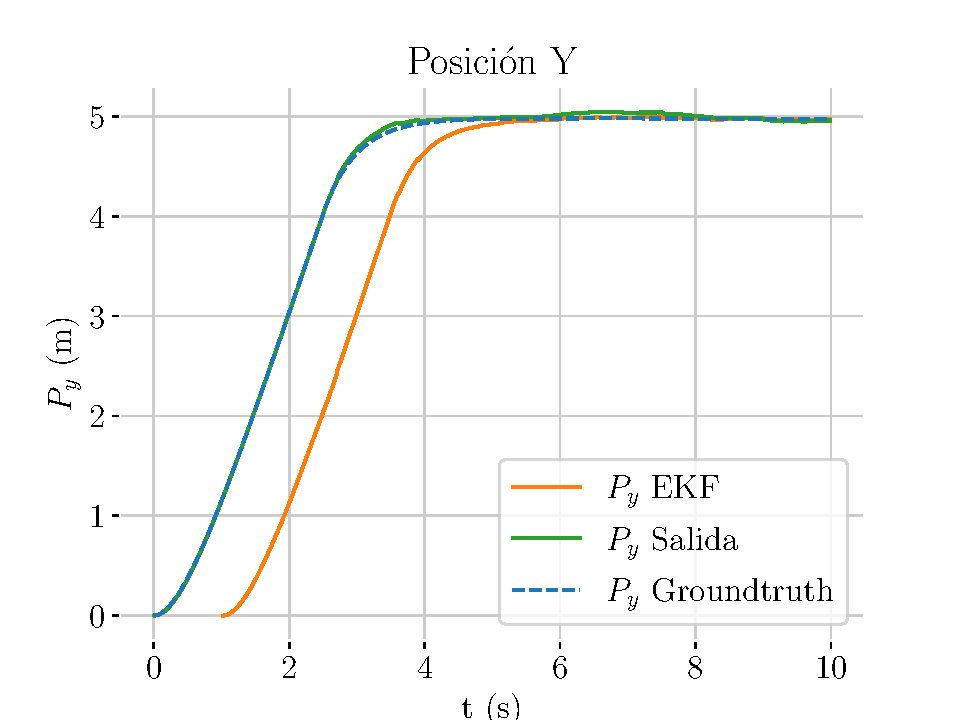
\includegraphics[width=\textwidth]{estimador_px4/im_simu/handle_delay/y_t}
		\caption{}
		\label{fig:handle-yt}		
	\end{subfigure}
	\quad
	\hspace*{-0.5cm}
	\begin{subfigure}[t]{0.49\textwidth}
		\centering
		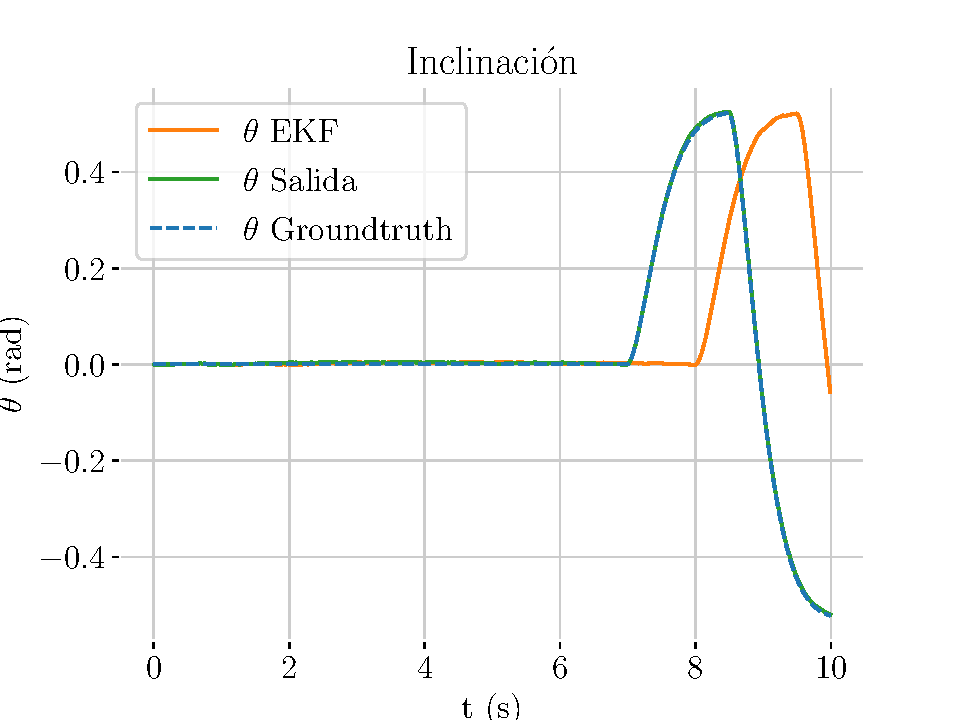
\includegraphics[width=\textwidth]{estimador_px4/im_simu/handle_delay/theta}
		\caption{}
		\label{fig:handle-theta}		
	\end{subfigure}
	\quad
	\begin{subfigure}[t]{0.49\textwidth}
		\centering
		\includegraphics[width=\textwidth]{estimador_px4/im_simu/handle_delay/vx}
		\caption{}
		\label{fig:handle-vx}		
	\end{subfigure}
	\quad
	\caption{Experimento con manejo de medidas retrasadas}\label{fig:handle}
\end{figure}





\endinput


\begin{appendices}
\chapter{Simulador del estimador de estados}\label{chp:simu}

El siguiente archivo también puede verse y descargarse en el repositorio \url{https://github.com/isidroas/quadrotor\_simulator}

%\begin{codigo}{Simulador del estimador de estados  (\textit{main.py})}
\inputminted[bgcolor=black!5!white]{python}{apendices/quadrotor_simulator/main.py}
%\end{codigo} 

\chapter{Detector de marcadores visuales}

Los siguientes archivos se encuentran también en \url{https://github.com/isidroas/rpi\_vision\_uav}

\section{main.cpp}
\inputminted[bgcolor=black!5!white]{c++}{apendices/rpi_vision_uav/main.cpp}

\section{vision\_params.yml}\label{sec:vision-params}
\inputminted[bgcolor=black!5!white]{yaml}{apendices/rpi_vision_uav/vision_params.yml}

\section{marker\_vision.h}

\newcounter{lineInvertPoseA}
\newcounter{lineInvertPoseB}
\setcounter{lineInvertPoseB}{291}
\setcounter{lineInvertPoseA}{\thelineInvertPoseB -7}

\inputminted[bgcolor=black!5!white,lastline=\thelineInvertPoseA]{c++}{apendices/rpi_vision_uav/marker_vision.h}

La siguiente función invierte la posición y la rotación. También corrige la posición de la cámara con respecto al UAV. Sus argumentos son:
\begin{itemize}
\item rvec.  Vector de entrada. Vector de rotación del marcador con respecto a los ejes de la cámara
\item tvec.  Vector de entrada. Translación del marcador con respecto a los ejes de la cámara
\item pos.   Vector de salida. Posición del uav/cámara con respecto al marcador
\item eul.   Vector de salida. Orientación del uav con respecto al marcador. El orden de los elementos son 0: roll, 1: pitch, 2: yaw
\end{itemize}

\inputminted[bgcolor=black!5!white,firstline=\thelineInvertPoseB]{c++}{apendices/rpi_vision_uav/marker_vision.h}

\section{mavlink\_helper.h}
\inputminted[bgcolor=black!5!white]{c++}{apendices/rpi_vision_uav/mavlink_helper.h}
 
\end{appendices}

%%:Empieza todo lo que no constituye el cuerpo en si del libro. Todo lo que va detrás
\backmatter

%:Indice de figuras, coméntese las siguientes líneas si no se desea
\cleardoublepage
\phantomsection

%:Para añadir una línea en blanco en el TOC y separar esta lista
\addtocontents{toc}{\protect\mbox{}\protect\hspace*{0pt}\par}
\addcontentsline{toc}{listasb}{\listfigurename}
\pagestyle{especial}
\listoffigures

%:Indice de tablas, coméntese las siguientes líneas si no se desea
\cleardoublepage
\phantomsection
\addcontentsline{toc}{listasb}{\listtablename}
\pagestyle{especial}
\listoftables

%:Indice de Programas
%\cleardoublepage
%\phantomsection
%\addcontentsline{toc}{listasb}{\lstlistlistingname}
%\pagestyle{especial}
%\lstlistoflistings

%:Bibliografía con biblatex y biber
\cleardoublepage
\phantomsection
\addcontentsline{toc}{listasb}{\bibname}
\pagestyle{especial}
%BIBER
\printbibliography[heading=etsi]

%:Índice alfabético de palabras
\cleardoublepage
\phantomsection
\addcontentsline{toc}{listasb}{\indexname}
\chaptermark{\indexname}
\printindex


%:Acrónimos
%\cleardoublepage
%\phantomsection
%\addcontentsline{toc}{listasb}{\glossaryname}
%\chaptermark{\glossaryname}
%\printglossaries

\end{document}
